\section{The \sparc{} Assembly Language}
\label{sec:modeling}

\begin{figure*}[!t]
	\centering
	\small
	\[
		\begin{array}{rcclcrccl}
			\TYPE{(Word)} & \word, \lab{} & \in & 
			\multicolumn{6}{l}
			{ 
				\TYPE{Int32} \qquad
				\TYPE{(Block)} \ \block \, \in \, \Ztype 
				\qquad
				\TYPE{(Addr)} \ \loc \, \in \,  
					\TYPE{Block} \times \TYPE{Word}
				\qquad
				\TYPE{(Val)} \ \val \,
					\define \, \word \sepline \loc
			}
			\\
			\\
			\TYPE{(Prog)} & \prog & \define & 
				(\code, \state, \pc, \npc) & \qquad & 
			\TYPE{(CodeHeap)} & \ \code \ & \in &  
				\TYPE{Word} \rightharpoonup \TYPE{Comm}
			\\
			\\[-8pt]
			\TYPE{(State)} & \state & \define & 
				(\mem, \Rstate, \DBuf) & & 
			\TYPE{(RState)} & \Rstate & \define & 
				(\RFile, \Wstack) 
			\\
			\\[-8pt]
			\TYPE{(Memory)} & \mem & \in & 
				\TYPE{Addr} \rightharpoonup \TYPE{Val} 
			& & 
			\TYPE{(ProgCount)} & \pc, \npc & \in & \TYPE{Word}
			\\
			\\[-8pt]
			\TYPE{(OpExp)} & \oexp & \define & 
				\reg{} \sepline \word & & 
			\TYPE{(AddrExp)} & \aexp & \define & 
				\oexp \sepline \reg{} + \oexp \\
			\\
			\TYPE{(Comm)} & \comm & \define & 
			\multicolumn{6}{l}
			{
				\simplins{} \sepline \call{} \ \lab{}
				\sepline \jmp{} \ \aexp \sepline \retl{} \sepline
				\be \ \lab{} 
			} \\
			\\[-8pt]
			\TYPE{(SimpIns)} & \simplins{} & \define & 
			\multicolumn{6}{l}
			{
				\ld{} \ \aexp \ \reg{d} \sepline 
				\st{} \ \reg{s} \ \aexp \sepline
				\nop{} \sepline  
				\cadd{} \ \reg{s} \ \oexp \ \reg{d} \sepline
				\csave{} \ \reg{s} \ \oexp \ \reg{d} \sepline 
				\crestore{} \ \reg{s} \ \oexp \ \reg{d}
			} \\
			& & \ \ \ \ | & 
			\multicolumn{6}{l}
			{
				\rd{} \ \sr \ \reg{d} \sepline 
				\cwr{} \ \reg{s} \ \oexp \ \sr \sepline
				\dots
			} \\ 
			\\[-8pt]
			\TYPE{(InstrSeq)} & \cblk & \define & 
			\multicolumn{6}{l}
			{
				\simplins{}; \, \cblk \sepline 
				\jmp{} \ \aexp; \, \simplins{} \sepline 
				\call{} \ \lab{}; \simplins{}; \cblk \sepline 
				\retl{} \ \simplins{} \sepline 
				\be{} \ \lab{}; \, \simplins{}; \, \cblk
			}
		\end{array}
	\]
	\vspace*{-0.5em}
	\caption{Machine States and Language for SPARCv8 Code}
	\label {fig:Machine States and Language for SPARC Code}
	\vspace*{-0.5em}
\end{figure*}

We introduce the key \sparc{} instructions, the model of machine
states, and the operational semantics in this section.

\subsection{Language syntax and states}
\label{subsec:syntax}
% \begin{figure*}[!t]
% 	\begin{tabular}{rcclcrccl}
% 		(Word) & $\, \word$, $\lab{} \, $ & $\in$ & Int32 & & 
% 		(Block) & $\block$ & $\in$ & $\Ztype$ \\
% 		(Addr) & $\loc$ & $\in$ & $\text{Block} \times \text{Word}$ 
% 		& & 
% 		(Val) & $\val$ & $\define$ & $\word \sepline \loc$
% 		\\[1.2ex]
		
% 		(Prog) & \prog & $\define$ & $(\code, \state, \pc, \npc)$ & $\quad\quad$ &
%         %(CodeHeap) & $\code$ & $\define$ & $\{\lab{} \rightsquigarrow c\}^*$ \\
%         (CodeHeap) & $\code$ & $\in$ & $\text{Word} \rightharpoonup \text{Comm}$ \\
		
% 		(State) & $\state$ & $\define$ & $(\mem, \Rstate, \DBuf)$ &$\quad\quad$&
%         (RState) & $\Rstate$ & $\define$ & $(\RFile, \Wstack)$ \\
		
% 		(Memory) & $\mem$ & $\in$ & $\text{Addr} \rightharpoonup \text{Val}$ & $\quad\quad$ &
% 		(ProgCount) & \pc, \npc & $\in$ & Word \\
		
% 		(OpExp) & $\oexp$ & $\define$ & $\regr \sepline \word$ & &
%         (AddrExp) & $\aexp$ & $\define$ & $\oexp \sepline \regr+\oexp$ \\[1ex]
		
% 		%(Value) & $w, v, \cwp$ & $\in$ & Word & & & & & \\
		
% 		(Comm) & $c$ & $\define$ &
% 		\multicolumn{6}{l}
% 		{$\simplins \sepline
% 		   \call \; \lab{} \sepline
% 		   \jmp \; \aexp \sepline
% 		   \retl \sepline
% 		   \be \; \lab{} $} \\
		
% 		(SimpIns) & $\simplins$ & $\define$ &
% 		\multicolumn{6}{l}
% 		{$\ld \; \aexp \; \reg{d} \sepline
% 			\st \; \reg{s} \; \aexp \sepline
% 			\nop \sepline
% 			\csave \; \reg{s} \; \oexp \; \reg{d} \sepline
% 			\crestore \; \reg{s} \; \oexp \; \reg{d}  $} \\
% 		& & \ \, $\sepline$ &
% 		\multicolumn{6}{l}
% 		{$\cadd \; \reg{s} \; \oexp \; \reg{d} \sepline
% 			\rd \; \sr \; \reg{d} \sepline
% 			\cwr \; \reg{s} \; \oexp \; \sr \sepline
% 			\dots$} \\
		
% 		(InstrSeq) & $\cblk$ & $\define$ &
% 		\multicolumn{6}{l}
% 		{$\simplins; \, \cblk \sepline
% 			\jmp \; \aexp; \simplins \sepline
% 			\call \; \lab{}; \, \simplins; \cblk \sepline
% 			\retl; \, \simplins \sepline
% 			\be \; \lab{}; \; \simplins; \, \cblk$}
		
% 	\end{tabular}
% 	\caption{Machine States and Language for SPARCv8 Code}
% 	\label {fig:Machine States and Language for SPARC Code}
% \end{figure*}

The machine model and syntax of \sparc{} assembly language
are defined in Fig.~\ref{fig:Machine States and Language for SPARC Code}. 
Here, we follow the block-based memory \cite{CompCertMM} introduced 
in CompCert to define the memory in our work.   
% so that each procedure can have a block of its own 
% stack frame. 
The memory address $\loc$ is defined as a pair of 
its block id and the offset. The type of block is the integer 
in mathemantics represent as $\Ztype$, and the type of offset 
is a 32-bit integer, which we called {\it words} in our work. 
So, the value here is either a word $\word$ or address $\loc$.  
The whole program configuration $\prog$ consists of the code heap
$\code$, the machine state $\state$, and the program counters $\pc$
and $\npc$.
%\sparc{} program can be viewed as a composition of
%code heap, machine state, pc and npc.
The code heap $\code$ is a partial function
from labels $\lab{}$ to commands $c$.
Labels are also 32-bit integers (called {\em words}),
which can be viewed as addresses or locations 
where the commands are saved in code heap. 
The operand expression $\oexp$, which is either a general 
register $\reg{}$ or a word $\word$, 
and address expression $\aexp$, 
which is either a operand expression or a 
sum of the value of register $\reg{}$ and an operation 
expression, are auxiliary definitions used as paramters of commands. 
Commands in \sparc{} can be classified into two categories,
the simple instructions $\simplins$ and the
control-transfer instructions like $\call$ and $\jmp$.

The machine state $\state$ consists of three parts:
the memory $\mem$, the register state $\Rstate$
which is a pair of register file $\RFile$ and frame list $\Wstack$,
and the delay buffer $\DBuf$.
As defined in Fig.~\ref{fig:Register File and Frame List},
$\RFile$ is a partial mapping
from register names to values.
Registers include the general registers $\regr$,
the processor state register $\psr$
and the special registers $\sr$.
The processor state register $\psr$ contains
the integer condition code fields $\regn$,
$\regz$, $\regv$ and $\regc$,
which can be modified by the arithmetic and logical instructions
and used for conditional control-transfer,
and $\regcwp$ recording the id of the current register window.
We explain the frame list $\Wstack$ and the delay buffer
$\DBuf$ below.

\begin{figure*}[!t]
	\small
	\begin{tabular}{rcclcrccl}
		(RegFile) & $\RFile$ & $\in$ & $\text{RegName} \rightharpoonup 
			\text{Val}$

         & $\quad$ &
        (RegName) & $\regN$ & $\define$ &
         $\reg{0} \sepline \dots \sepline \reg{31} \sepline \psr \sepline \sr$ \\
		
		%(GenReg) & $r$ & $\define$ &
		%$\reg{0} \sepline \dots \sepline \reg{31}$ & $\quad\quad$ &
		(PsrReg) & $\psr$ & $\define$ &
		$\regn \sepline
			\regz \sepline
			\regv \sepline
			\regc \sepline \regcwp$ & $\quad$ &
        %		
		(SpeReg) & $\sr$ & $\define$ &
		$\regwim \sepline
			\regY \sepline
\asr_0 \sepline \dots \sepline \asr_{31}$ \\
		
		(FrameList) & $\Wstack$ & $\define$ &
                            $\nil \sepline \fm \stCons \Wstack$ & $\quad$ &
		(Frame) & $\fm$ & := & $[\val_0, \dots, \val_7]$ \\
		
		(DelayBuff) & $\DBuf$ & $\define$ & $\nil \sepline
                                  (\tick, \sr, \word) \dbCons \DBuf$
                                  & $\quad$
                                  %& & & & \\		
		%(DelayItem) & $d$ & $\define$ & $(\tick, \sr, \word)$ & $\quad$
		& (DelayCycle) & $\tick$ & $\in$ & $\{ 0, 1, \dots, X \}$
	\end{tabular}
	\caption{Register File, Frame List and DelayBuffer}
	\label{fig:Register File and Frame List}
\end{figure*}

\begin{figure*}[!t]
	\centering
	%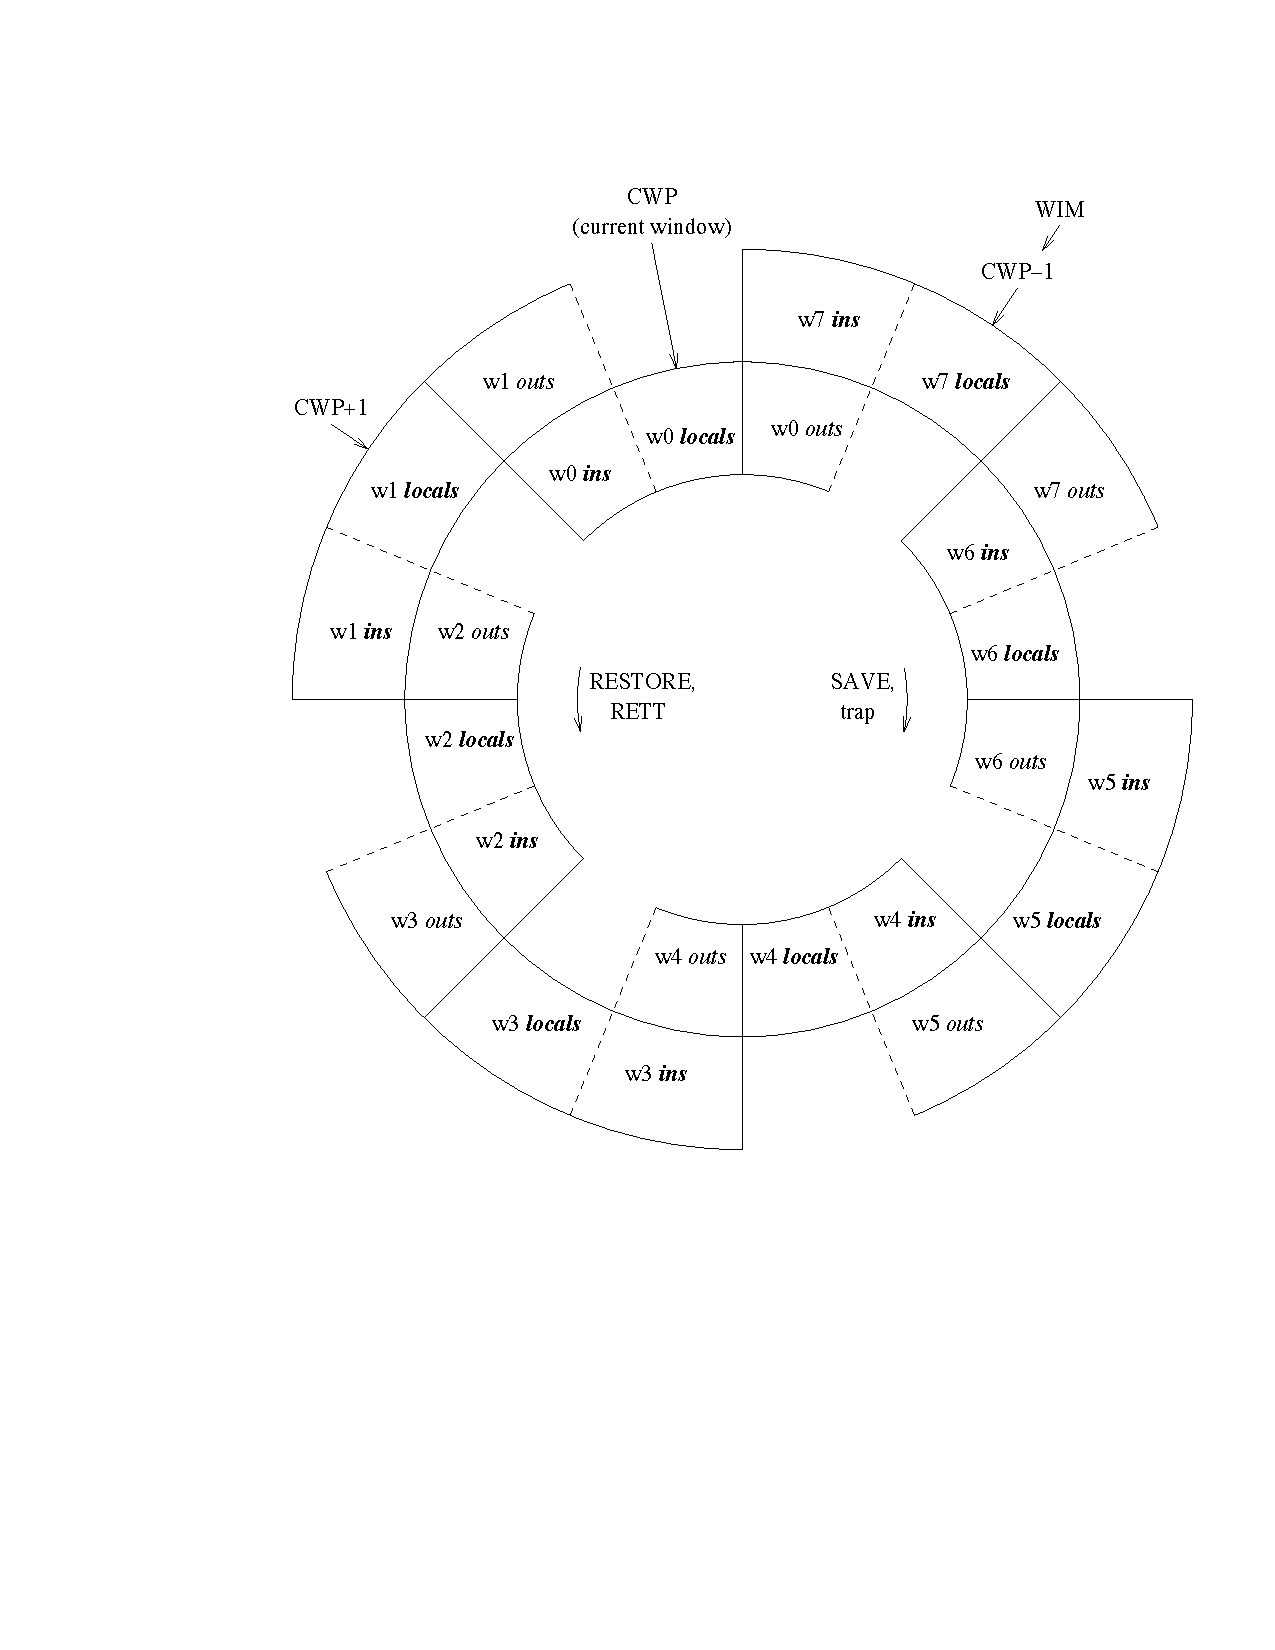
\includegraphics[width=63ex]{window}
	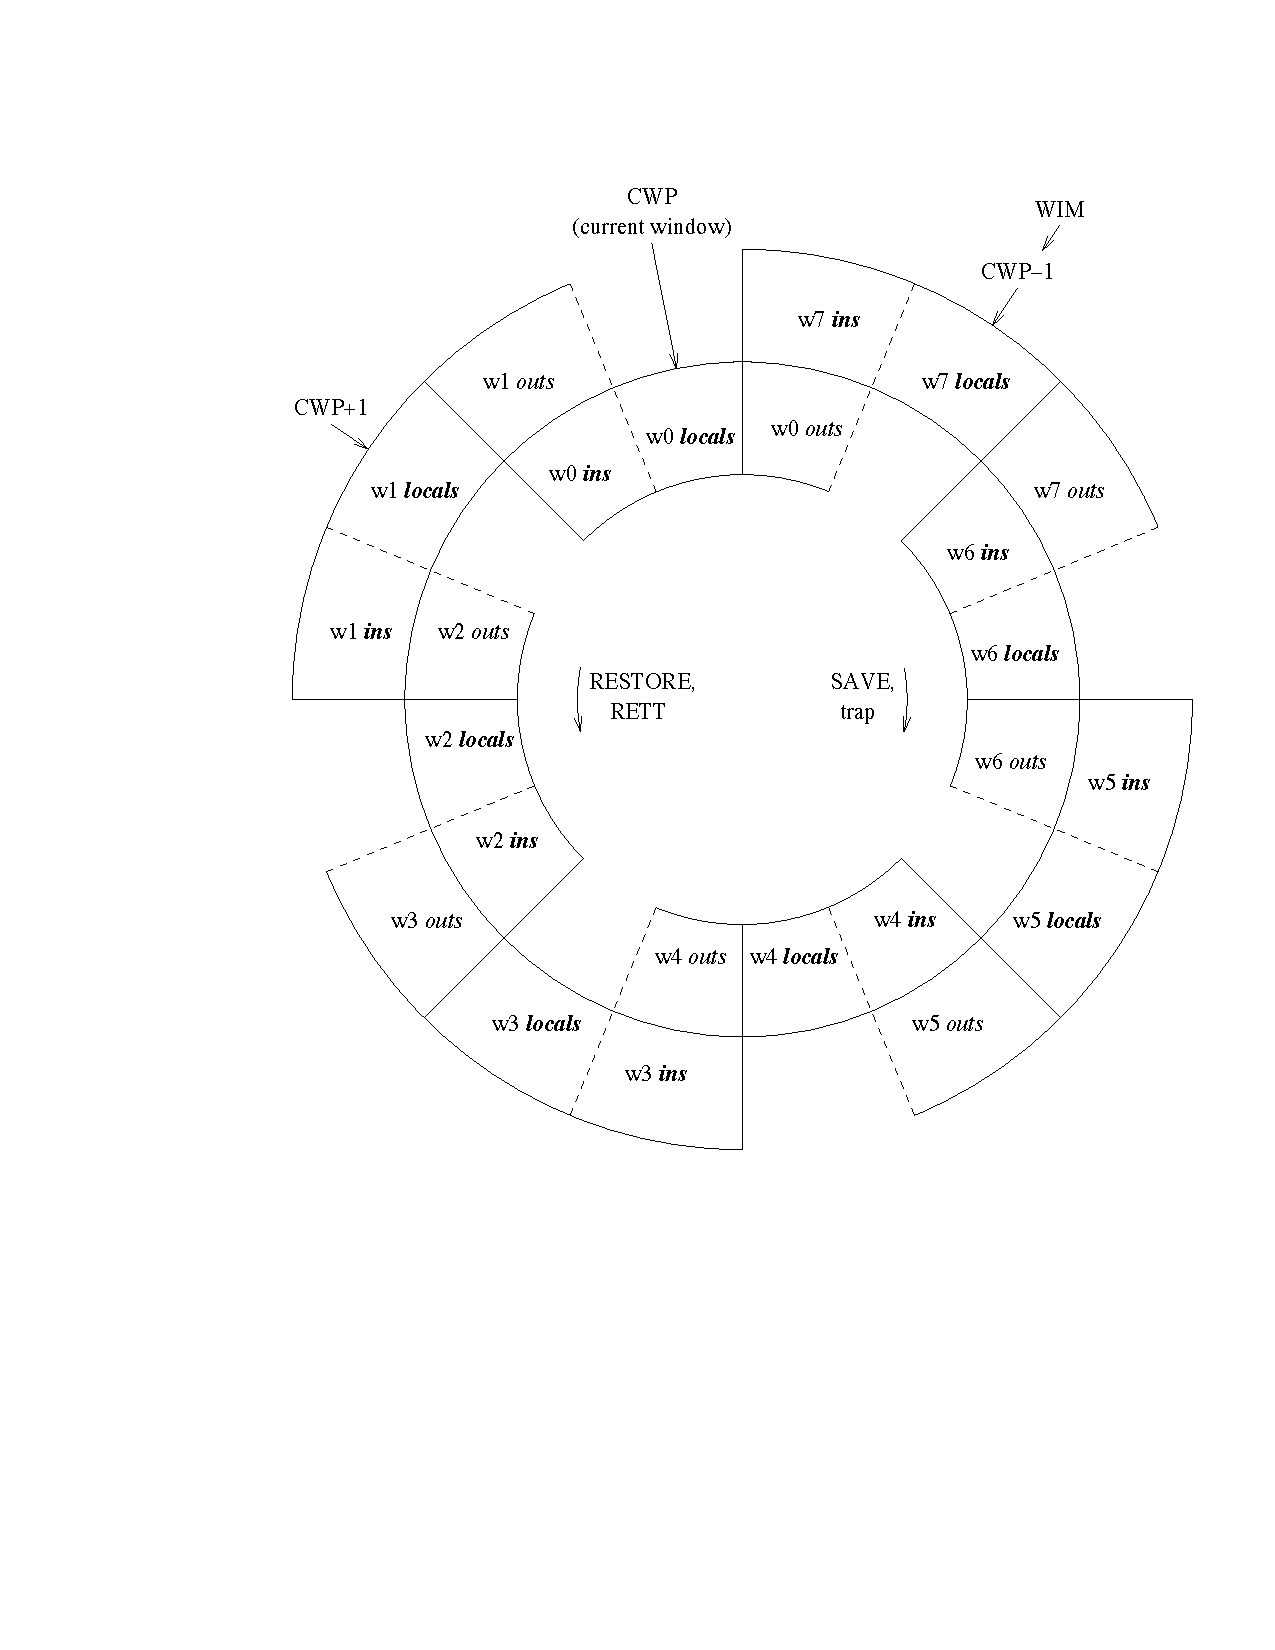
\includegraphics[width=54ex]{window}
	\caption{Register Windows (figure taken from \cite{sparc})}
	\label{fig:RegisterWindows}
\end{figure*}

\paragraph{\textbf{Register windows and frame List.}}
\sparc{} provides 32 general registers, which are split into
four groups
as \globalRN{} ($\reg{0} \sim \reg{7}$),
\outRN{} ($\reg{8} \sim \reg{15}$), \localRN ($\reg{16} \sim \reg{23}$)
and \inRN{} ($\reg{24} \sim \reg{31}$) registers.
The latter three groups (\outRN{}, \localRN{} and \inRN{})
form the current {\em register window}.
% \begin{center}
% 	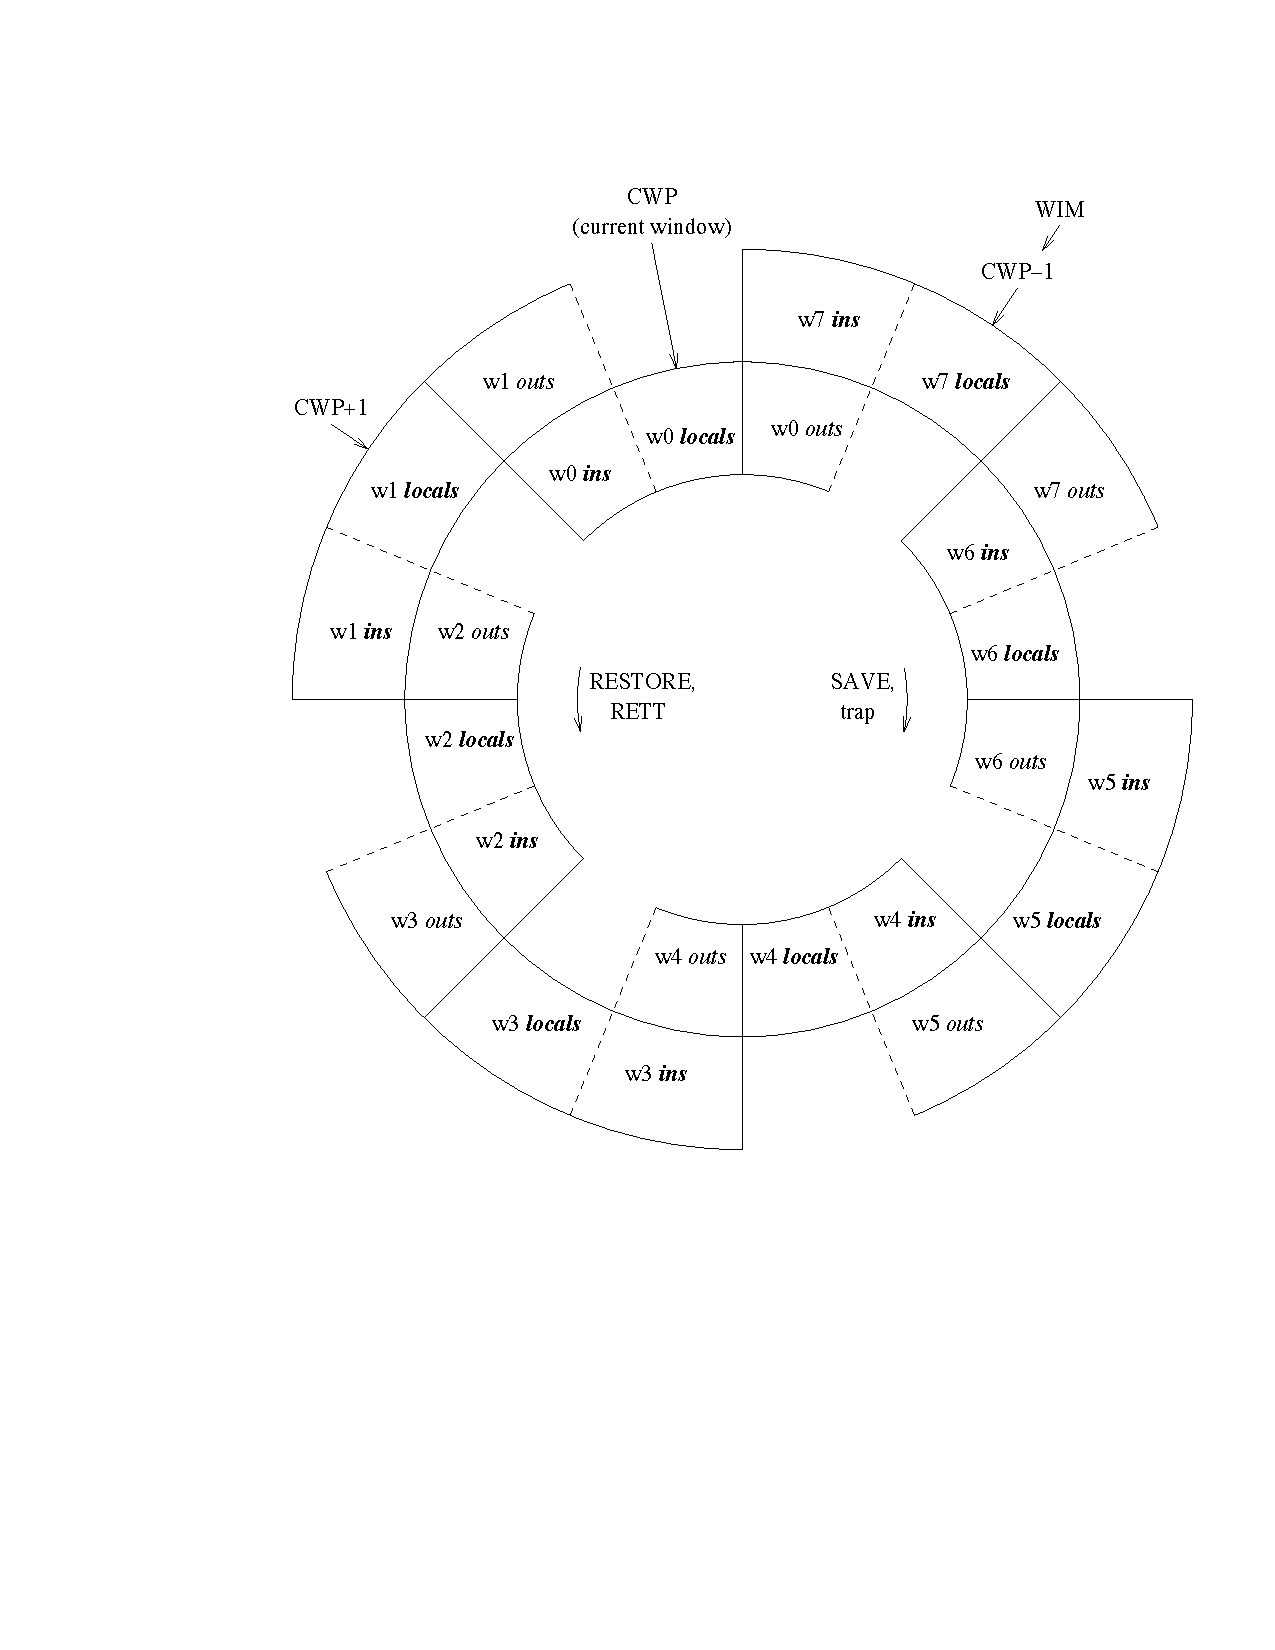
\includegraphics[width=60ex]{window}
% 	\figurecaption{Register Windows (figure taken from \cite{sparc})}
% 	\label{fig:RegisterWindows}
% \end{center}

At the entry and exit of functions and traps, one may need to
save and restore some of the general registers as execution
contexts. Instead of saving them into stacks in memory,
\sparc{} uses multiple register windows to form a circular
stack, and does window rotation for efficient context save and restore.
As shown in Fig.~\ref{fig:RegisterWindows}, there are $N$
register windows ($N=8$ here) consisting of $2\times N$
groups of registers (each group containing 8 registers).
The $\regcwp$ register (part of $\psr$) records the id number
of the current window ($\regcwp=0$ in this example).

The \inRN{} and \outRN{} registers of each window are shared
with its adjacent windows for parameter passing.
For example, the \inRN{} registers of the $\text{w}_0$
is the \outRN{} registers of the $\text{w}_1$,
and the \outRN{} registers of the $\text{w}_0$
is the \inRN{} registers of the $\text{w}_7$.
This explains
why we need only $2\times N$ groups of registers for
$N$ windows, while each window consisting of
three groups (\outRN{}, \localRN{} and \inRN{}).


\begin{figure*}[!t]
    \[
     \begin{array}{l}
     \outRN \ \define \  [\reg{8}, \dots, \reg{15}]
     \qquad
     \localRN \ \define \  [\reg{16}, \dots, \reg{23}] %
      \qquad
     \inRN \ \define \  [\reg{24}, \dots, \reg{31}]
     \\
     \\[-8pt]
     \RFile([\reg{i}, \dots, \reg{i+k}]) \ \define\
     [\RFile(\reg{i}), \dots, \RFile(\reg{i+k})]
     \\
     \\[-8pt]
     %
     \Rupd{\reg{i}, \dots, \reg{i+7}}{\fm} \ \define \
			R\{ \reg{i} \rightsquigarrow \val_0 \} 
				\dots \{ \reg{i+7} \rightsquigarrow \val_7 \} \\
            \hspace*{28ex}\text{where }\ \ \fm = [\val_0, \dots, \val_7]
     \\
     \\ %[-8pt]
     %
     %\qquad \Rlocal \ \define\ [\RFile(\reg{8}), \dots, \RFile(\reg{15})] \\

        \begin{array}{lcl}
            \winvalid(\cwp, \RFile) & \define & 2^{\cwp}
                                            \,\bitAND\, \RFile(\regwim) = 0 \\
             & & \ \ \ \mbox{where $\bitAND$ is the bitwise AND operation.}
            \\
            \\[-8pt]
		    \precwp(\cwp) & \define & (\cwp + N - 1) \modOP N
            %\\
		    %\\[-8pt]
            \qquad\quad
		    \postcwp(\cwp) \ \define \ (\cwp + 1) \modOP N
        \end{array}
            \\
		    \\ %[-8pt]
            %
        \begin{array}{lcl}
            \decwin(\RFile, \Wstack) & \define &
            \left\{
            \begin{array}{ll}
                (\RFile', \Wstack')
                & \quad \textit{if }
                             \cwp' = \precwp(\RFile(\regcwp)),
                             \winvalid(\cwp', \RFile), \\
                & \quad \ \ \
                             \Wstack = \Wstack'' \lstApp \fm_1 \lstApp \fm_2, \
                              \Wstack' = \RFile(\localRN)
                                          \stCons\RFile(\inRN)\stCons\Wstack'',\\
                & \quad \ \ \ \RFile'' =
                \RFile\{\inRN\rightsquigarrow \RFile(\outRN),
                        \localRN\rightsquigarrow \fm_2,
                        \outRN \rightsquigarrow \fm_1\},
                \\
                 & \quad \ \ \
                            \RFile' = \fsubst{\RFile''}\regcwp{\cwp'},
                 \\
                 %
                \perp &\quad \textit{if }
                                  \lnot\winvalid(\precwp(R(\regcwp)), \RFile)
            \end{array}
            \right. \\
%            & & \where \ \ Q = (R, F)
            \\
            \\[-8pt]

            \incwin(\RFile, \Wstack) & \define &
            \left\{
            \begin{array}{ll}
                (\RFile', \Wstack')
                & \quad \textit{if }
                             \cwp' = \postcwp(\RFile(\regcwp)),
                             \winvalid(\cwp', \RFile), \\
                & \quad \ \ \
                             \Wstack = \fm_1 \stCons \fm_2 \stCons \Wstack''  , \
                              \Wstack' = \Wstack''\lstApp \RFile(\outRN)
                                                  \lstApp \RFile(\localRN), \\
                                          %\stCons\RFile(\inRN)\stCons\Wstack''\\
                & \quad \ \ \ \RFile'' =
                \RFile\{\inRN\rightsquigarrow \fm_2,
                        \localRN\rightsquigarrow \fm_1,
                        \outRN \rightsquigarrow \RFile(\inRN)\},
                \\
                 & \quad \ \ \
                            \RFile' = \fsubst{\RFile''}\regcwp{\cwp'},
                 \\
                 %
                \perp &\quad \textit{if }
                                  \lnot\winvalid(\postcwp(R(\regcwp)), \RFile)
            \end{array}
            \right.
        \end{array}
    \end{array}
    \]
    \caption{Auxiliary Definitions for Instruction \csave{} and \crestore}
    \label{fig:save and restore}
\end{figure*}

To save the context, the $\csave$ instruction
rotates the window by decrements the $\regcwp$ pointer
(modulo $N$).
So $\text{w}_7$ becomes the current window. The \outRN{}
registers of $\text{w}_0$ becomes
the \inRN{} registers of $\text{w}_7$.
The \inRN{} and \localRN{} registers of $\text{w}_0$
become inaccessible.
This is like pushing them
onto the circular stack.
The $\crestore$ instruction does the inverse, which is like
a stack pop.

The $\regwim$ register is used as a bit vector to record the
end of the stack. Each bit in $\regwim$ corresponds to a
register window. The bit corresponding to the last available
window is set to 1, which means {\em invalid}. All other bits
are 0 ({\em i.e. valid}).
%Given a window pointer $\cwp$ in $\regcwp$,
When executing $\csave$ (and $\crestore$), we need to ensure
the next window is valid, in order to avoid the overflow 
of register window because of the limitation of the number 
of windows. We use the assertion $\winvalid(\cwp, \RFile)$ defined
in Fig.~\ref{fig:save and restore} to say the
window pointed to by $\cwp$ is valid, given the value of
$\regwim$ in $\RFile$.
%$$
%\winvalid(\cwp, \RFile) \ \define \ 2^{\cwp}  \& \RFile(\regwim) = 0
%$$
%where $\&$ represents bitwise AND.

We use the frame list $\Wstack$ to model the circular stack consisting
of register windows. As defined in Fig.~\ref{fig:Register File and Frame List},
a frame is an array of 8 words, modeling a group of 8 registers.
$\Wstack$ consists of a sequence of frames corresponding to all the
register windows except the \outRN{}, \localRN{} and \inRN{}
registers in the current window. Then $\csave$ saves the
\localRN{} and \inRN{} registers onto the head of $\Wstack$
and loads the two groups of register at the {\em tail} of $\Wstack$
to the \localRN{} and \outRN{} registers (and the original
\outRN{} registers becomes the \inRN{} group). The $\crestore$
instruction does the inverse. The operations are defined formally
in Fig.~\ref{fig:save and restore}.

\paragraph{\textbf{The delay buffer.}}
The delay buffer $\DBuf$ is a sequence of delayed writes.
Because the  $\cwr$ instruction
does not update the target register immediately,
we put the write operation onto the delay buffer.
A delayed write is recorded as a triple consisting of
the remaining cycles $\tick$ to be delayed,
the target special register $\sr$ and the value 
$\word$ to be written. Note that we restrict that 
the value of a special register can only be a word, 
because the special registers are used to record the 
state of processor, and there is impossible to 
store memory addresses in them.  

\paragraph{\textbf{Instruction sequences.}}
%\indent \indent
We use an instruction sequence $\cblk$ to model
a basic block, \ie{} a sequence of commands ending
with a control transfer.
As defined in Fig.~\ref{fig:Machine States and Language for SPARC Code},
we require that a delayed control-transfer instruction
must be followed by  a simple instruction $\simplins$,
because the actual control-transfer occurs after
the execution of $\simplins$.
The end of each instruction sequence can only be
$\jmp$ or $\retl$  followed by a simple
instruction $\simplins$.
Note that we do not view the $\call$ instruction
as the end of a basic block, since the callee is
expected to return, following our direct-style
semantics for function calls.
We define $\code[\lab{}]$ to extract 
an instruction sequence starting 
from $\lab{}$ in $\code$ below.
\[
	\small
	C[\lab{}] =
	\left\{
		\begin{array}{ll}
			\simplins; \cblk &
			\quad \ \ \code(\lab{}) = \simplins \; 
				\text{and} \; \code[\lab{}+4] = \cblk \\
			
			\\[-8pt]
			
			\comm; \simplins &
			\quad \ \ 
				\comm = \code(\lab{}) \; \text{and} \; 
				\comm = \jmp \; \aexp \; \text{or} \; \retl
			\\ & \quad \ \ \text{and} \; C(\lab{}+4) = \simplins \\
			
			\\[-8pt]
			
			\comm; \simplins; \cblk &
			\quad \ \ \comm = \code(\lab{}) \; 
			\text{and} \; c = \call \; \lab{} \; \text{or} \; \be \; \lab{} \\
			& \quad \ \ \text{and} \; 
				\code(\lab{}+4) = \simplins \; \text{and} \;
				\code[\lab{}+8] = \cblk \\
			
			\\[-8pt]
			
			\undef & \quad \ \ \text{otherwise}
		\end{array}
	\right.
\]

\subsection{Operational Semantics}
\label{subsec : Operational Semantics}

\begin{figure*}
	\centering
	\vspace{-0.5em}
	\subfigure[Program Transistion]
	{
		\begin{minipage}[b]{1\textwidth}
		\small
		\[
			\infer
			{
				\ptrans{((M, (R, F), D), \pc, \npc)}
					{((M', (R'', F'), D''), \pc', \npc')}
			}
			{
				\begin{array}{l}
					%\exedelay(R, D) = (R', D') \\
					\Dstep{(R, D)}{(R', D')} \\
					\cttrans{((M, (R', F), D'), \pc, \npc)}
						{((M', (R'', F'), D''), \pc', \npc')}
				\end{array}
			}
		\]
		\vspace{0.05cm}
		\end{minipage}
	}
	
	\subfigure[Control Transfer Instruction Transition]
	{	
		\begin{minipage}[b]{1\textwidth}
		\small
        \[
            \infer
            {
                \cttrans{((M, (R, F), D), \pc, \npc)}
                    {((M', (R', F'), D'), \npc, \npc+4)}
            }
            {
                \code(\pc) = \simplins \quad \quad
                    \swtrans{(M, (R, F), D)}{\; \; \simplins \; \;}{(M', (R', F'), D')}
            }
        \]

		\[
			\infer
			{
				\cttrans{((M, (R, F), D), \pc, \npc)}
					{((M, (R, F), D), \npc, \lab{})}
			}
			{
				C(\pc) = \jmp \; \aexp \quad \; \;
				\eval{\aexp} = \lab{}
			}
		\]
		
		\[
			\infer
			{
				\cttrans{((M, (R, F), D), \pc, \npc)}
				{
					((M, (R\{\reg{15} \rightsquigarrow \pc\}, F), D), \text{npc}, \lab{})
				}
			}
			{
				C(\pc) = \call \; \lab{} \quad \; \;
					\reg{15} \in \text{dom}(R)
			}			
		\]
		
		\[
			\infer
			{
				\cttrans{((M, (R, F), D), \pc, \npc)}
				{
					((M, (R, F), D), \text{npc}, \lab{}\!+\!8)
				}
			}
			{
				C(\pc) = \retl \quad R(\reg{15}) = \lab{}
			}
		\]
		\vspace{0.05cm}
		\end{minipage}
	}
	
	\subfigure[Save, Restore and Wr instruction Transition]
	{
		\begin{minipage}[b]{1\textwidth}
			\small
			\begin{minipage}{0.48\textwidth}
			\[
				\infer
				{
					\swtrans{(M, (R, F), D)}{\; \; \simplins \; \;}
						{(M', (R', F), D)}
				}
				{
					\itrans{(M, R)}{\simplins}{(M', R')}
				}
			\]
			\end{minipage}
			\begin{minipage}{0.48\textwidth}
				\[
					\infer
					{
						\swtrans{(M, (R, F), D)}
						{\cwr \; \reg{s} \; \oexp \; \sr}{(M, (R, F), D')}
					}
					{
						\begin{array}{l}
							R(\reg{s}) = \word_1 \quad \; \;
							{\llbracket \oexp \rrbracket}_R = \word_2 \quad \; \;
							w = \word_1 \!\xorOP\! \word_2 \\
							\sr \in \text{dom}(R) \quad \; \; D' = \textbf{set\_delay}(\sr, w, D)
						\end{array}
					}
				\]
			\end{minipage}

            \centering
            \vspace{0.3cm}
            \begin{minipage}{1\textwidth}
                \infer
                {
                    \swtrans{(\Mem, (\RFile, \Wstack), \DBuf)}
                    {\csave \; \reg{s} \; \oexp \; \reg{d}}
                    {(\Mem, (\RFile'', \Wstack'), \DBuf)}
                }
                {
					\decwin{(\RFile, \Wstack)} = 
						(\RFile', \Wstack') \quad
                    \eval{\oexp} = \val
					\quad
					\val' = \RFile(\reg{s}) \!+\! \val
					\quad
                    \RFile'' =
                      \fsubst{\RFile'}{\reg{d}}{\val'}
                }
                \vspace{0.3cm}
                \infer
                {
                    \swtrans{(\Mem, (\RFile, \Wstack), \DBuf)}
                    {\crestore \; \reg{s} \; \oexp \; \reg{d}}
                    {(\Mem, (\RFile'', \Wstack'), \DBuf)}
                }
                {
                    \incwin{(\RFile, \Wstack)} = (\RFile', \Wstack') \quad
                    \eval{\oexp} = \val
					\quad
					\val' = \RFile(\reg{s}) \!+\! \val
					\quad
                    \RFile'' =
                      \fsubst{\RFile'}{\reg{d}}{\val'}
                    %R'' = R'\{ \reg{d} \rightsquigarrow \eval{\reg{s}} + \word \}
                }
            \end{minipage}
			
			\vspace{0.3cm}
		\end{minipage}
	}
	
	\subfigure[Simple Instruction Transition]
	{
		\begin{minipage}[b]{1\linewidth}
			\small
			\begin{minipage}{0.5\linewidth}
				\[
					\infer
					{
						\itrans{(M, R)}{\rd \; \sr \; \reg{d}}
							{(M, R\{ \reg{d} \rightsquigarrow \word \})}
					}
					{
						R(\sr) = \word \quad \ \ \reg{d} \in \dom(R)
					}
				\]
			\end{minipage}
			\begin{minipage}{0.5\linewidth}
				\[
					\infer
					{
						\itrans{(M, R)}{\cadd \; \reg{s} \; \oexp \; \reg{d}}
						{
							(M, R\{\reg{d}
                                 \rightsquigarrow \val\})	
						}
					}
					{
						R(\reg{s}) = \val_1 \quad
						{\llbracket \oexp \rrbracket}_R = \val_2 \quad
						\val = \val_1\!+\!\val_2 \quad
						\reg{d} \in \text{dom}(R)
					}
				\]
			\end{minipage}
			
			\vspace{0.2cm}
			\centering
			\begin{minipage}{1\textwidth}
				\[
					\infer
					{
						\itrans{(M, R)}{\ld \; \aexp \; \reg{d}}
						{(M, R\{\reg{d} \rightsquigarrow \val'\})}
					}
					{
						{\llbracket \aexp \rrbracket}_R = \loc \quad
						%\textbf{word\_align}(w) \quad
                        M(\loc) = \val' \quad
						\reg{d} \in \text{dom}(R)
					}
				\]
			\end{minipage}
			\vspace{0.3cm}
		\end{minipage}	
	}

	\subfigure[Expression Semantics]
	{
		\begin{minipage}[b]{1\linewidth}
			\small
            $$
            \begin{array}{ll}
                \begin{array}{lcl}
                    \evalR{\oexp}{R} & \define &
                    \left\{
                        \begin{array}{ll}
                            R(r) &\quad \cif \ \oexp = r \\
                            \\[-8pt]
                            w &\quad \cif \ \oexp = \word, \\
                            & \quad \quad -4096 \leq \word \leq 4095 \\
                            \\[-8pt]
                            \perp &\quad \otherwise
                        \end{array}
                    \right.
                \end{array} & \quad
                \begin{array}{lcl}
                    \evalR{\aexp}{R} & \define &
                    \left\{
                        \begin{array}{ll}
                            \evalR{\oexp}{R} &\quad \cif \ \aexp = \oexp \\
                            \\[-8pt]

                            \val_1 \!+\! \val_2
                              &\quad \cif \ \aexp = \regr \!+\! \oexp,\
                              R(\regr) \!=\! \val_1 \\
                            & \quad \quad \tand \ \evalR{\oexp}{R} = \val_2 \\

                            \\[-8pt]
                            \perp &\quad \otherwise
                        \end{array}
                    \right.
                \end{array}
            \end{array}
            $$
			\vspace{0.3cm}
		\end{minipage}	
	}
	\caption{Selected operational semantics rules}
	\label{Selected Operational Semantics}
\end{figure*}

The operational semantics is taken from 
\etal{Wang}~\cite{sparc-formalization},
but we use block-based memory model and 
omit features like interrupts and traps.
We show the selected rules in Fig.~\ref{Selected Operational Semantics}.
The program transition relation 
$\ptrans{(\state, \pc, \npc)}{(\state', \pc', \npc')}$
is defined 
in Fig.~\ref{Selected Operational Semantics} (a).
Before the execution of the instruction pointed by
$\pc$, the delayed writes
in $\DBuf$ with $0$ delay cycles are executed first.
The execution of the delayed writes are defined in the
form of $\Dstep{(\RFile, \DBuf)}{(\RFile', \DBuf')}$ below:

{\small
$$
\begin{array}{c}
\infer
{\Dstep{(\RFile, \nil)}{(\RFile,\nil)}}
{}
\\
\\
%
% \qquad\qquad
%
\infer
{\Dstep{(\RFile, (\tick\!+\!1, \sr, \word)\dbCons\DBuf)}
       {(\RFile', (\tick, \sr, \word)\dbCons\DBuf')}}
{\Dstep{(\RFile, \DBuf)}{(\RFile', \DBuf')}}
\\
\\
\infer
{\Dstep{(\RFile, (0, \sr, \word)\dbCons\DBuf)}{(\fsubst{\RFile'}\sr\word, \DBuf')}}
{\Dstep{(\RFile, \DBuf)}{(\RFile', \DBuf')}
\qquad \sr\in\dom(\RFile)
}
%
% \qquad\qquad
\\
\\
%
\infer
{\Dstep{(\RFile, (0, \sr, \word)\dbCons\DBuf)}{(\RFile', \DBuf')}}
{\Dstep{(\RFile, \DBuf)}{(\RFile', \DBuf')}
 \qquad \sr\not\in\dom(\RFile)
}
\end{array}
$$
}

Note that the write of $\sr$ has no effect if $\sr$ is not
in the domain of $\RFile$. Since $\RFile$ is defined as a partial
map, we can prove the following lemma.
\begin{lemma}
    \em
	\label{lemma:RFileSplitExDelay}
	$\Dstep{(\RFile, \DBuf)}{(\RFile', \DBuf')}$
    and $\RFile = \RFile_1 \uplus \RFile_2$,
    if and only if
    there exists $\RFile_1'$ and $\RFile_2'$, such that
    $\Dstep{(\RFile_1, \DBuf)}{(\RFile_1', \DBuf')}$, $\Dstep{(\RFile_2, \DBuf)}{(\RFile_2', \DBuf')}$,
    and $\RFile' = \RFile_1' \uplus \RFile_2'$.
\end{lemma}
Here the disjoint union $\RFile_1 \uplus \RFile_2$ represents the union of
$\RFile_1$ and $\RFile_2$ if they have disjoint domains, and undefined
otherwise. This lemma is important to give sound semantics
to delay buffer related assertions, as discussed in
Sec.~\ref{sec:logic}.

%Although this would never happen
%at runtime, this feature is useful for giving sound semantics
%to delay buffer related assertions, as shown in Sec.~\ref{sec:logic}.

%We define the operation semantics of \sparc{} with multiply layers.
%We just select a part of transition rules
%in Fig. \ref{Selected Operational Semantics}
%to give readers a whole recognition for \sparc{} program execution
%because of the space limitation.
%As shown in Fig. \ref{Selected Operational Semantics},
%we define the operational semantics with four layers.
%As for the first layer Program Transition,
%we can see that
%a step of \sparc{} program transition can be split into two steps.
%The state transition ``$\Dstep{}{}$" checks each element in delay list,
%remove the delay items whose delay cycles are 0
%and write the value recorded in them to specific special register.
%Second, the instruction that \pc{} points executes.
%We define the state transition caused by delay list simply as following.
%We can find that if a special register $\sr$ recorded in $\DBuf$ isn't
%in the domain of $\RFile$. It will not make any changes for $\RFile$.

%\[
%	\small
%	\begin{array}{rcl}
%		\exedelay(R, D) & \define &
%		\left\{
%			\begin{array}{ll}
%				(R, D) & \quad  D = \nil \\
%				
%				\\[-8pt]
%				
%				(R'\{\sr \rightsquigarrow w\}, D'') & \quad D = (0, \sr, w) :: D', \\
%				& \quad \ \ (R', D'') = \exedelay(R, D') \\
%				
%				\\[-8pt]
%				
%				(R', (n-1, \sr, w) :: D'') & \quad D = (n, \sr, w) :: D', n > 0, \\
%				& \quad \ \ (R', D'') = \exedelay(R, D')
%			\end{array}
%		\right.
%	\end{array}
%\]

The transition steps for individual instructions are classified into
three categories: the control transfer steps 
($\ccttrans{\notCare}{\notCare}{\notCare}$), 
the steps for
$\csave$, $\crestore$ and $\cwr$ instructions 
($\swtrans{\notCare}{\ \notCare\ }{\notCare}$),
and the steps
for other simple instructions
($\itrans{\notCare}{\ \notCare\ }{\notCare}$). The
corresponding step transition relations are defined inductively 
in Fig.~\ref{Selected Operational Semantics} (b), (c) and (d)
respectively.

Note that, after the control-transfer instructions, $\pc$ is set
to $\npc$ and $\npc$ contains the target code pointer. This explains
the one cycle delay for the control transfer.
The $\call$ instruction saves $\pc$ into the register $\RAreg$,
while $\retl$ uses $\RAreg \!+\! 8$ as the
return address (which is the address for the second instruction
following the $\call$). Evaluation of
expressions $\aexp$ and $\oexp$ is defined
as 
% $\evalR\aexp\RFile$ 
and 
% $\evalR\oexp\RFile$
in Fig.~\ref{Selected Operational Semantics} (e). 
Here, we define the sum of two values $\val_1$ 
and $\val_2$ below. The result of $\val_1\!+\!\val_2$ 
is legel, if both of the $\val_1$ and $\val_2$ 
are words (Int32), or $\val_1$ is an address and 
$\val_2$ is an offset. The offset is a word, 
which acts as an immediate value in the 
calculation of address.
% This is explain why the 
% immediate value in our work is a word, because 
% immediate value usually acts as an offset, which 
% is a word, in the calculation of address. 
\[
	\small
	\val_1 + \val_2 \ \define \ 
	\left\{
		\begin{array}{ll}
			\word_1 + \word_2 & \quad \cif \  
				\val_1 = \word_1, \text{ and } 
				\val_2 = \word_2 \\
			\\[-8pt]
			(\block, \word_1 + \word_2) & \quad 
				\cif \ 
				\val_1 = (\block, \word_1), 
				\text{ and } 
				\val_2 = \word_2 \\
			\\[-8pt]
			\perp & \quad \otherwise
		\end{array}
	\right.
\]
%%addresses properly aligned on a 4-byte boundary
%
%The second layer Control Transfer Instruction Transition
%describes the change of pc and npc for each \sparc{} instruction execution.
%Transition rules for control-transfer instructions
%(e.g., \jmp, \call, \retl) are defined in this layer.
%We can see that delayed control-transfer instructions like $\call$
%will change $\npc$ instead of $\pc$ to target,
%set original $\npc$ to $\pc$
%and cause the control transfer delayed one cycle.
%The instruction $\retl$ and $\ret$ are two common instructions in \sparc{},
%which are used for function return.
%The instruction $\retl$ returns to the address of $\lab{}+8$
%(where $R(\reg{15}) = \lab{}$).
%However, the address used for return for instruction $\ret$ is
%saved in $\reg{31}$.
%The instruction $\ret$ is used for the situation that
%the procedure will execute an instruction $\csave$ and allocate a new window for itself.
%The instruction $\call$ stores its label in register $\reg{15}$,
%and instruction $\csave$ will let the original $\reg{15}$ become $\reg{31}$
%of the new window by window rotation.


The $\cwr$ wants to save the bitwise exclusive OR of
the operands into the special register $\sr$, but
it puts the write into the delay buffer $\DBuf$
instead of updating $\RFile$ immediately.
The operation $\setdelay(\sr, \word, \DBuf)$
is defined below:
\[
	\small
	\begin{array}{l}
		\setdelay(\sr, \word, D) \define (X, \sr, \word) 
		\dbCons \DBuf \\
	\end{array}
\]
where $X$ ($0 \leq X \leq 3$) is a
predefined system parameter for the delay cycle. 
% Note that 
% as we have explained before, special register is used 
% to record the state of processors, so we do not permit saving 
% memory address in it. 
%whose specific value is implementation dependently.

The $\csave$ and $\crestore$ instruction rotate
the register windows and update the register file.
Their operations over $\Wstack$ and $\RFile$
are defined in Fig.~\ref{fig:save and restore}.

%Instruction $\csave$, $\crestore$ and $\cwr$
%are different with the other simple instructions
%because they may change the state of frame list and delay list.
%And we present their transition in the third layer.
%The rule for instruction $\cwr$ tells us
%that the \sparc{} set the write operation in delay list
%instead of updating the value of target special register $\sr$ immediately.
%The operation of $\setdelay(\sr, w, D)$ is defined as following,
%where $X$ ($0 \leq X \leq 3$) is the delay cycle
%whose specific value is implementation dependently :
%\[
%	\small
%	\begin{array}{l}
%		\setdelay(\sr, w, D) \define (X, \sr, w) :: D \\
%	\end{array}
%\]
%
%
%\indent
%The execution of instruction \csave{} and \crestore{} will cause the
%window rotation, so that will change the state of Frame List $F$.
%The operation $\decwin{(R, F)}$ describe that, if previous window is valid,
%we will do a right rotation for register windows by $\rightwin(R, F)$.
%As for instruction \crestore{}, it will change the register window by
%$\incwin{(R, F)}$, which will do a left rotation by $\leftwin(R, F)$ for register window.
%The auxiliary definitions for operational semantics of \csave{} and \crestore{}
%are shown in Fig. \ref{fig:save and restore}.
%
%\indent
%The last layer is designed for some simple instructions,
%whose executions only touch memory and register file.
